\documentclass{article}
\usepackage{graphicx} % Required for inserting images
\usepackage[a4paper,margin=1in]{geometry}
\usepackage[T1]{fontenc}
\usepackage{lmodern}
\usepackage{graphicx}
\usepackage{setspace}
\usepackage{parskip}
\usepackage{hyperref}
\usepackage{booktabs}
\usepackage{titling}

\title{Beyond 4/4: A Fairness Study of Time Signature Control in Text-to-Music Generation }
\author{Qicheng Jin (qjin5), Kevin Liu (kevinl25)}
\date{May 2026}

\begin{document}
\setlength{\droptitle}{-8.5em} 
\maketitle
\vspace{-1.5em}                

\section{Introduction}

This project studies the fairness issues in text-to-music generation models through the lens of time signature control. 

\subsection{what is time signature}

When you listen to music, you can usually feel a repeating pulse, like a heartbeat. The time signature tells you how many of those pulses are grouped together before the pattern repeats. For "twinkle twinkle little star", you count 1-2-3-4, 1-2-3-4, and that's a 4/4. For "We Wish You A Merry Christmas", you count 1-2-3, 1-2-3, and that's a 3/4. If you are familiar with the "Mission: Impossible" theme, that's a 5/4, which is rare and most text-to-music generation models will fail. To describe time signature formally, it defines how beats are grouped in each repeating cycle (for example, 4/4 means four beats per bar, 3/4 means three beats per bar, and 5/4 means five beats per bar). 

\subsection{intention of study}

The rhythm is a core part in music. For downstream tasks like composition, film scoring, or game audios require strict time signature constraints. Models that fail to generalize beyond 4/4 also reflect a cultural bias. If models inherently treat 4/4 as a default, it will marginalize traditions that rely on other time signatures, for example waltz(3/4), some jazz(5/4), and Irish jigs(6/8). 

This project investigates two dimensions of the bias:
User-experience bias: whether colloquial/cultural prompts including genre labels (waltz), cultural descriptions (Balkan folk) or reference-based("a jazz song like 'take five'") are handled better than formal music-theory prompts (explicitly specifying required time signature e.g. “3/4 time,” “6/8 time”). 
Cultural bias: whether models tend to collapse non-4/4 targets into 4/4, which may under-represent musical traditions that rely on other meters.



\section{Experiments}

\subsection{model selection}
We select two text-to-music models to experiment: suno-v4.5, a state-of-the-art music generation model from Suno,  and Lyria 3,  Google's most recent text-to-music model, which has been integrated directly into Gemini now. 

\subsection{prompt design}
We created paired prompts for each target time signature so that each pair had similar instrumentation, mood, and style, and differed mainly in phrasing style:

Cultural prompt: uses common musical language (genre/tradition terms).

Formal prompt: explicitly states the time signature in notation.


\begin{tabular}{p{2cm} p{6.2cm} p{6.2cm}}
\toprule
\textbf{Meter} & \textbf{Cultural Prompt} & \textbf{Formal Prompt} \\
\midrule

2/4 &
``An energetic march with brass and snare drums.'' &
``An energetic piece in 2/4 time with brass and snare drums.'' \\

3/4 &
``A dramatic waltz with full orchestra and sweeping strings.'' &
``A dramatic piece in 3/4 time with full orchestra and sweeping strings.'' \\

\bottomrule
\end{tabular}
\\
% The distinction between cultural and formal prompts in this study is specifically defined as: whether the time signature is communicated implicitly through genre/tradition labels versus explicitly stated in music-theory notation.

Target meters in this study are: 2/4, 3/4, 4/4, 5/4, and 6/8.
For each meter, we wrote 5 prompt pairs to reduce prompt-specific randomness and improve robustness.

\subsection{labeling}
We use madmom, a python package for music information retrieval (e.g., beat/downbeat and meter analysis), to automatically do time signature labeling, then, samples with confidence < 0.9 are manually reviewed by human. 

\section{Results}

\subsection{Overall accuracies across time signatures}
Both suno and lyria perform best on generate 4/4 music, getting $100\%$ accuracy for both cultural and formal prompts. Then, 2/4 are the second best for both models, Lyria got $100\%$ and Suno got $70\%$. In contrast, for 3/4, 6/8, and especially 5/4, both models show limited capability to generate music in the required time signature. 
% \begin{figure}[htbp]
%     \centering
%     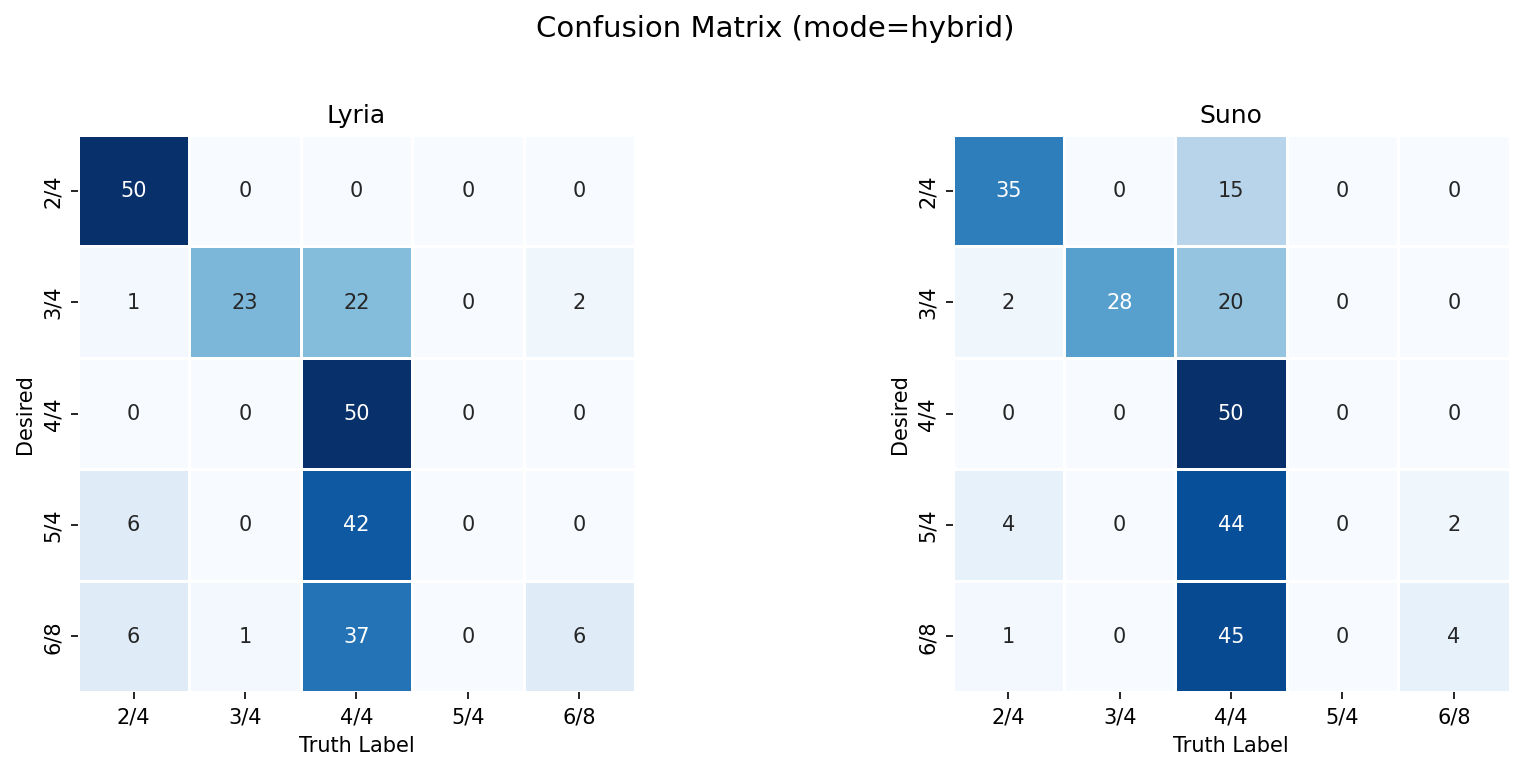
\includegraphics[width=0.9\textwidth]{figures/confusion_matrix_hybrid.png}
%     \caption{Confusion matrix}
%     \label{fig:confusion_hybrid}
% \end{figure}

\subsection{Do models respond differently to cultural and formal prompts?}

As shown in Figure~\ref{fig:rq1_hybrid}, we observe small accuracy gaps between cultural and formal prompts in certain meters: $4\%$ in Lyria 3/4, $4\%$ in Suno 2/4, and $8\%$ in Suno 6/8. Fisher's exact tests were performed for each time signature to assess whether these differences are statistically significant. Overall, there are visual gaps in performance for some time signatures but none of the observed differences show statistical significance, likely due to limited sample size. Therefore, the conclusion is that models treat two types of prompts indifferently, such that the user-experience bias is not supported by the data.

\begin{figure}[htbp]
    \centering
    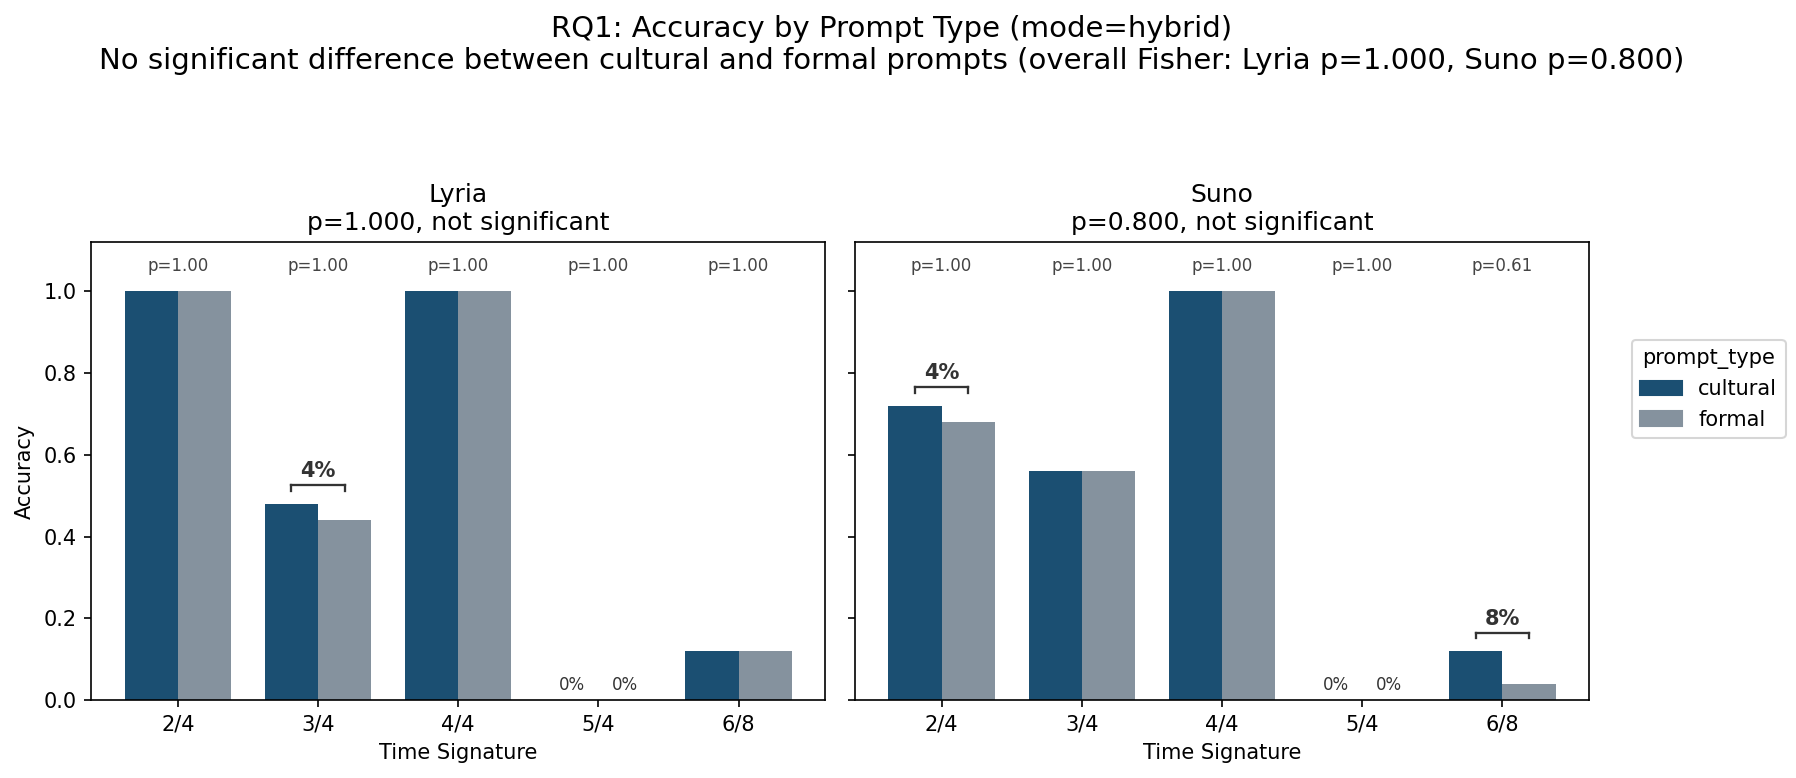
\includegraphics[width=0.9\textwidth]{figures/rq1_prompt_type_hybrid.png}
    \caption{Accuracy by prompt type (cultural vs. formal)}
    \label{fig:rq1_hybrid}
\end{figure}


\subsection{do models collapse non-4/4 Time signatures to 4/4?}

As shown in Figure~\ref{fig:rq2_hybrid}, we observe clear collapse patterns from non-4/4 targets to 4/4, especially for 5/4 and 6/8.  
For Lyria, the collapse-to-4/4 rates are about $44\%$ (3/4), $84\%$ (5/4), and $74\%$ (6/8).  
For Suno, the collapse rates are about $40\%$ (3/4), $88\%$ (5/4), and $90\%$ (6/8). In contrast, 2/4 shows much lower collapse rates (Lyria $0\%$, Suno $30\%$). Overall, this pattern is strongest in 5/4 and 6/8, where collapse dominates over correct generation. Therefore, the results support the cultural-bias concern in the sense that less common time signatures are systematically under-produced and collapse to 4/4.


\begin{figure}[htbp]
    \centering
    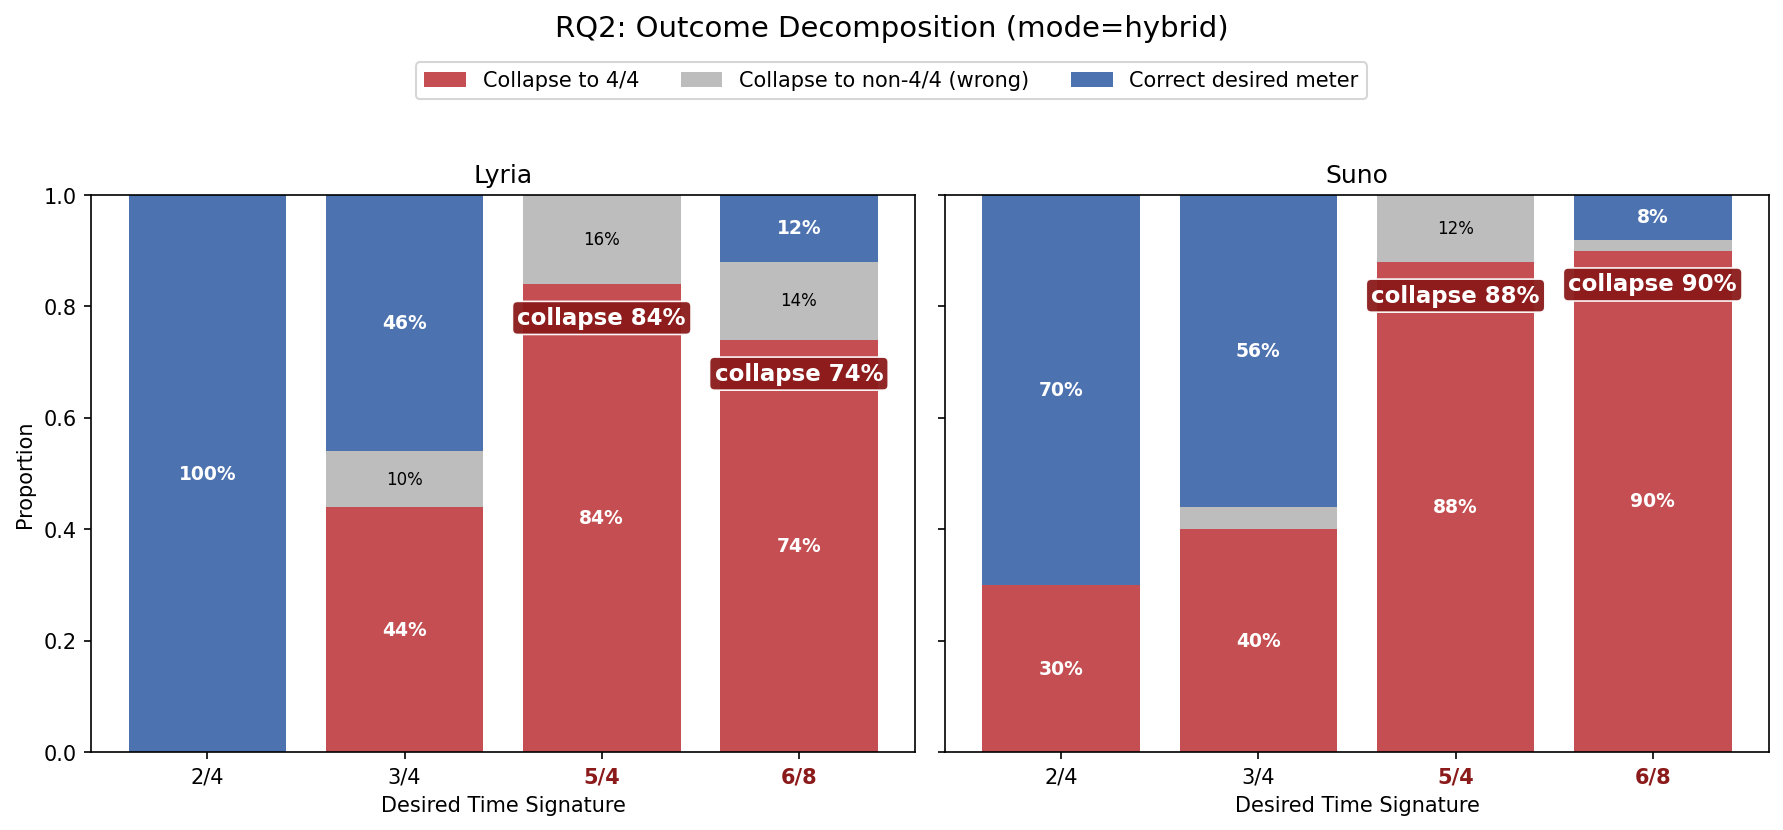
\includegraphics[width=0.9\textwidth]{figures/rq2_collapse_hybrid.png}
    \caption{Collapse-to-4/4 rate for non-4/4 targets under hybrid labeling.}
    \label{fig:rq2_hybrid}
\end{figure}


\section{Discussion}
Based on the results above, user-experience bias is not supported by the data, while we do find evidence of cultural bias: time signatures other than 4/4 are underrepresented, and many outputs tend to collapse to 4/4. That raises fairness concerns: 

First, musical cultures that rely on less common time signatures are more likely to be marginalized when models collapse outputs into 4/4.  
Examples include:
\begin{itemize}
    \item \textbf{5/4 jazz traditions}, often referenced by works such as \textit{Take Five};
    \item \textbf{6/8 Irish traditions}, where compound meter is a core rhythmic identity;
\end{itemize}

When these time signatures are systematically mapped to 4/4, the model does not simply make random mistakes; it reproduces a narrower musical representation and reduces rhythmic diversity in generated music.

Second, this has user-level consequences across different backgrounds.  
For users from communities where non-4/4 time signatures are common, the model may provide lower-quality service for culturally meaningful requests.  
For musicians and producers who need specific time signatures for composition, arrangement, dance alignment, or scoring, collapse to 4/4 increases  prompting difficulty and their extra efforts to edit.
In practice, users who request mainstream 4/4 styles are better served than users requesting rhythmically distinctive traditions, which reflects an unequal distribution of model performance. 


\section{Limitations}
Several limitations should be noted. 

First, the sample size is relatively small: 250 generated songs per model, constrained by API costs (10 dollars for Lyria 3 and 10 dollars/month for Suno). This may explain why some observed differences, such as the $8\%$ gap in Suno 6/8, did not reach statistical significance.

Second, this study only evaluates two models. While Suno and Lyria 3 are representative of current state-of-the-arts, the findings may not generalize to other text-to-music models. 

Third, the prompting set only covers a small number of music traditions, many non-4/4 traditions such as 7/8 Balkan music, 9/8 slip jigs, or polyrhythmic West African styles are not directly tested. Also, we do not consider the case where time signature shifts across different sections of the song. 

\section{Conclusion}
This project examined fairness in text-to-music generation through time-signature control. Using a hybrid labeling pipeline (manual review for low-confidence cases and automatic labels otherwise), we compared Suno and Lyria across 2/4, 3/4, 4/4, 5/4, and 6/8.

Our findings show that both models perform well on common time signatures (especially 4/4), but struggle on less common ones. We did not find statistically significant evidence of user-experience bias between cultural and formal prompts. However, we found clear evidence of cultural bias in output behavior: non-4/4 targets, particularly 5/4 and 6/8, frequently collapse to 4/4.

Overall, current text-to-music systems provide uneven rhythmic coverage across musical traditions. Improving robustness on non-4/4 meters is important for both model quality and fairness.


\section{Project link}
The project repository is available at:

\url{https://github.com/QiChengJin/DATA359-final-project.git}

The code implementation, experiment scripts, and full prompt list are provided in this repository.

\end{document}
